% ------------------------------------------------------------------------
% ------------------------------------------------------------------------
% abnTeX2: Modelo de Trabalho Academico (tese de doutorado, dissertacao de
% mestrado e trabalhos monograficos em geral) em conformidade com
% ABNT NBR 14724:2011: Informacao e documentacao - Trabalhos academicos -
% Apresentacao
% ------------------------------------------------------------------------
% ------------------------------------------------------------------------

\documentclass[
	% -- opções da classe memoir --
	12pt,				% tamanho da fonte
	openright,			% capítulos começam em pág ímpar (insere página vazia caso preciso)
	twoside,			% para impressão em recto e verso. Oposto a oneside
	a4paper,			% tamanho do papel.
	% -- opções da classe abntex2 --
	%chapter=TITLE,		% títulos de capítulos convertidos em letras maiúsculas
	%section=TITLE,		% títulos de seções convertidos em letras maiúsculas
	%subsection=TITLE,	% títulos de subseções convertidos em letras maiúsculas
	%subsubsection=TITLE,% títulos de subsubseções convertidos em letras maiúsculas
	% -- opções do pacote babel --
	english,			% idioma adicional para hifenização
	brazil,				% o último idioma é o principal do documento
	svgnames
	]{abntex2}\usepackage[]{graphicx}\usepackage[]{color}
% maxwidth is the original width if it is less than linewidth
% otherwise use linewidth (to make sure the graphics do not exceed the margin)
\makeatletter
\def\maxwidth{ %
  \ifdim\Gin@nat@width>\linewidth
    \linewidth
  \else
    \Gin@nat@width
  \fi
}
\makeatother

\definecolor{fgcolor}{rgb}{0.345, 0.345, 0.345}
\newcommand{\hlnum}[1]{\textcolor[rgb]{0.686,0.059,0.569}{#1}}%
\newcommand{\hlstr}[1]{\textcolor[rgb]{0.192,0.494,0.8}{#1}}%
\newcommand{\hlcom}[1]{\textcolor[rgb]{0.678,0.584,0.686}{\textit{#1}}}%
\newcommand{\hlopt}[1]{\textcolor[rgb]{0,0,0}{#1}}%
\newcommand{\hlstd}[1]{\textcolor[rgb]{0.345,0.345,0.345}{#1}}%
\newcommand{\hlkwa}[1]{\textcolor[rgb]{0.161,0.373,0.58}{\textbf{#1}}}%
\newcommand{\hlkwb}[1]{\textcolor[rgb]{0.69,0.353,0.396}{#1}}%
\newcommand{\hlkwc}[1]{\textcolor[rgb]{0.333,0.667,0.333}{#1}}%
\newcommand{\hlkwd}[1]{\textcolor[rgb]{0.737,0.353,0.396}{\textbf{#1}}}%
\let\hlipl\hlkwb

\usepackage{framed}
\makeatletter
\newenvironment{kframe}{%
 \def\at@end@of@kframe{}%
 \ifinner\ifhmode%
  \def\at@end@of@kframe{\end{minipage}}%
  \begin{minipage}{\columnwidth}%
 \fi\fi%
 \def\FrameCommand##1{\hskip\@totalleftmargin \hskip-\fboxsep
 \colorbox{shadecolor}{##1}\hskip-\fboxsep
     % There is no \\@totalrightmargin, so:
     \hskip-\linewidth \hskip-\@totalleftmargin \hskip\columnwidth}%
 \MakeFramed {\advance\hsize-\width
   \@totalleftmargin\z@ \linewidth\hsize
   \@setminipage}}%
 {\par\unskip\endMakeFramed%
 \at@end@of@kframe}
\makeatother

\definecolor{shadecolor}{rgb}{.97, .97, .97}
\definecolor{messagecolor}{rgb}{0, 0, 0}
\definecolor{warningcolor}{rgb}{1, 0, 1}
\definecolor{errorcolor}{rgb}{1, 0, 0}
\newenvironment{knitrout}{}{} % an empty environment to be redefined in TeX

\usepackage{alltt}

% ---
% Novo list of (listings) para QUADROS
% ---

%\newcommand{\quadroname}{Quadro}
%\newcommand{\listofquadrosname}{Lista de quadros}

%\newfloat[chapter]{quadro}{loq}{\quadroname}
%\newlistof{listofquadros}{loq}{\listofquadrosname}
%\newlistentry{quadro}{loq}{0}

% configurações para atender às regras da ABNT
%\counterwithout{quadro}{chapter}
%\renewcommand{\cftquadroname}{\quadroname\space}
%\renewcommand*{\cftquadroaftersnum}{\hfill--\hfill}

% ---
% PACOTES
% ---
\usepackage{lscape}

\usepackage{listings}
\lstset{
  language=Python,
  basicstyle=\ttfamily\small,
  keywordstyle=\color{blue},
  stringstyle=\color{blue},
  commentstyle=\color{red},
  extendedchars=true,
  showspaces=false,
  showstringspaces=false,
  numbers=left,
  numberstyle=\tiny,
  breaklines=true,
  backgroundcolor=\color{green!10},
  breakautoindent=true,
  captionpos=b,
  xleftmargin=0pt,
}


% ---
% Pacotes fundamentais
% ---
\usepackage{lmodern}			% Usa a fonte Latin Modern
\usepackage[T1]{fontenc}		% Selecao de codigos de fonte.
\usepackage[utf8]{inputenc}		% Codificacao do documento (conversão automática dos acentos)
\usepackage{indentfirst}		% Indenta o primeiro parágrafo de cada seção.
\usepackage{color}			% Controle das cores
\usepackage{graphicx}			% Inclusão de gráficos
\usepackage{microtype} 			% para melhorias de justificação
\usepackage{setspace}
\usepackage{wrapfig}

% ---
% Para titulo em destaque sem sequencia de numeração
% ---
\newcommand{\datatitle}[1]{
  \normalsize \textsc{#1}
}

% ---
% Funções matematicas
% ---
\usepackage{amsmath,amssymb,amstext}
\usepackage{mathtools}                  % Funcionalidades (como \dcases)
\usepackage{dsfont}    %% Para \mathds{1} Indicadora
\usepackage{bm}

\DeclareMathOperator{\Ell}{\mathcal{L}}
\DeclareMathOperator{\R}{\mathbb{R}}
\DeclareMathOperator{\ind}{\mathds{1}}

\DeclareRobustCommand{\rchi}{{\mathpalette\irchi\relax}}
\newcommand{\irchi}[2]{\raisebox{\depth}{$#1\chi$}}

% ---
% Para tabelas
% ---
\usepackage{multirow}
\usepackage{array}
\usepackage{threeparttable}

% ---
% Pacotes e definições adcionais, para adequações especificas
% ---
\usepackage{tikz}
\usepackage{pdflscape}			% para ambiente landscape
\usepackage{pgfgantt}			% cronograma estilo gráfico de gantt
\usepackage{multicol}
\usetikzlibrary{backgrounds}
\usepackage{tasks}

% ---
% Fontes matemáticas
% ---
\usepackage{mathpazo}
\usepackage{inconsolata}
\usepackage{verbatim}

% ---
% Pacotes adicionais, usados apenas no âmbito do Modelo Canônico do abnteX2
% ---
\usepackage{lipsum}				% para geração de dummy text
% ---

% ---
% Pacotes de citações
% ---
\usepackage[brazilian,hyperpageref]{backref}% Paginas com as citações
\usepackage[alf, abnt-etal-list=0]{abntex2cite}				% Citações padrão ABNT

% ---
% CONFIGURAÇÕES DE PACOTES
% ---

% ---
% Configurações do pacote backref
% Usado sem a opção hyperpageref de backref
\renewcommand{\backrefpagesname}{Citado na(s) página(s):~}
% Texto padrão antes do número das páginas
\renewcommand{\backref}{}
% Define os textos da citação
\renewcommand*{\backrefalt}[4]{
  \ifcase #1 %
  Nenhuma citação no texto.%
  \or
  Citado na página #2.%
  \else
  Citado #1 vezes nas páginas #2.%
  \fi}%
% ---

% ---
% Informações de dados para CAPA e FOLHA DE ROSTO
% ---
\titulo{Aprendizado de máquina \\ Laboratório 3 - CNN}
\vspace{2cm}
\autor{Lineu Alberto Cavazani de Freitas}
\local{Curitiba}
\data{2021}
\instituicao{Universidade Federal do Paraná}

\preambulo{Relatório apresentado à disciplina
    Aprendizado de Máquina, ministrada pelo professor Luiz Eduardo Soares de Oliveira, no Programa de Pós Graduação em Informática da Universidade Federal do Paraná.}
% ---

% ---
% Configurações de aparência do PDF final

% informações do PDF
\makeatletter
\hypersetup{
  % pagebackref=true,
  pdftitle={\@title},
  pdfauthor={\@author},
  pdfsubject={\imprimirpreambulo},
  pdfcreator={LaTeX with abnTeX2},
  % pdfkeywords={abnt}{latex}{abntex}{abntex2}{projeto de pesquisa},
  colorlinks=true,	% false: boxed links; true: colored links
  linkcolor=blue,     % color of internal links
  citecolor=blue, % color of links to bibliography
  filecolor=magenta, % color of file links
  urlcolor=black,
  bookmarksdepth=4
}
\addto\captionsbrazil{
  \renewcommand{\bibname}{REFER\^ENCIAS}
}
\makeatother
% ---

% ---
% Espaçamentos entre linhas e parágrafos
% ---

% O tamanho do parágrafo é dado por:
\setlength{\parindent}{1.3cm}

% Controle do espaçamento entre um parágrafo e outro:
\setlength{\parskip}{0.2cm}  % tente também \onelineskip

% ---
% Highlight knitr code (pode-usar usar os varios highligths já definidos
% com thm = knit_theme$get("nuvola"); knit_theme$set(thm))
% ---

\renewcommand{\hlnum}[1]{\textcolor[rgb]{0.733,0,1}{#1}}%
\renewcommand{\hlstr}[1]{\textcolor[rgb]{0,0.533,0}{#1}}%
\renewcommand{\hlcom}[1]{\textcolor[rgb]{0,0,0}{#1}}%
\renewcommand{\hlopt}[1]{\textcolor[rgb]{0.412,0.412,0.412}{#1}}%
\renewcommand{\hlstd}[1]{\textcolor[rgb]{0.2,0.2,0.2}{{#1}}}%
\renewcommand{\hlkwa}[1]{\textcolor[rgb]{0.2,0.2,0.2}{{#1}}}%
\renewcommand{\hlkwb}[1]{\textcolor[rgb]{0.4,0,0}{\textbf{#1}}}%
\renewcommand{\hlkwc}[1]{\textcolor[rgb]{0.13,0.29,0.53}{#1}}%
\renewcommand{\hlkwd}[1]{\textcolor[rgb]{0.13,0.29,0.53}{\textbf{#1}}}%

% ---
% compila o indice
% ---
\makeindex
% ---

% ----
% Início do documento
% ----
\IfFileExists{upquote.sty}{\usepackage{upquote}}{}
\begin{document}

% Seleciona o idioma do documento (conforme pacotes do babel)
% \selectlanguage{english}
\selectlanguage{brazil}

% Retira espaço extra obsoleto entre as frases.
\frenchspacing

% ----------------------------------------------------------
% ELEMENTOS PRÉ-TEXTUAIS
% ----------------------------------------------------------
% \pretextual

% ---
% Capa
% ---
\tikz[remember picture,overlay] \node[opacity=1,inner sep=0pt] at
(current page.center){
  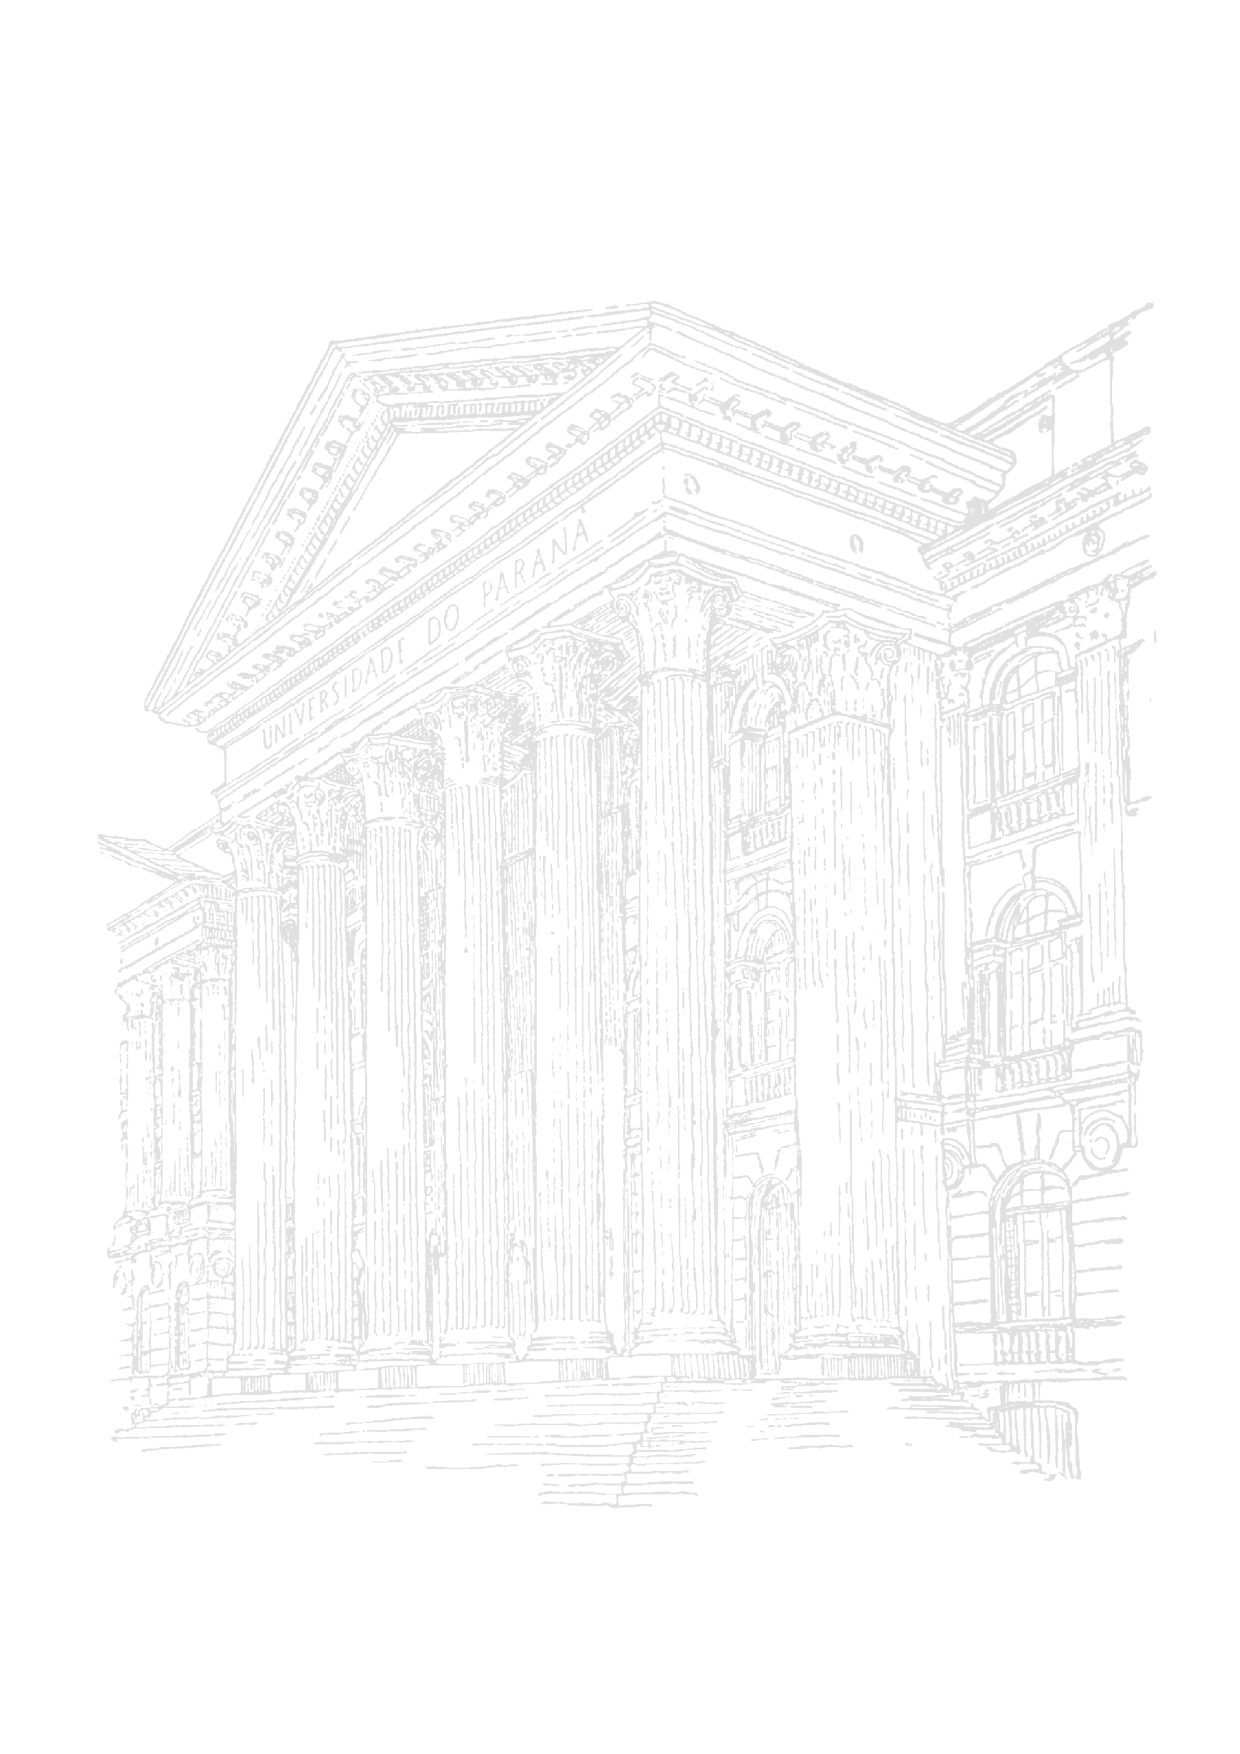
\includegraphics[width=\paperwidth,
  height=\paperheight]{images/ufpr_bg}};

\begin{center}
  {\Large \textsf{Universidade Federal do Paraná}}
  \vspace{-0.5cm}
\end{center}

\imprimircapa

% ---

% ---
% Folha de rosto
% ---
\imprimirfolhaderosto
% ---

% ---
% Dedicatória
% ---
% \begin{dedicatoria}
%   \lipsum[1]
% \end{dedicatoria}
% ---

% ---
% Agradecimentos
% ---
% \begin{agradecimentos}
%   \lipsum[1]
% \end{agradecimentos}
% ---

% ---
% Epígrafe
% ---
%\begin{epigrafe}
%    \vspace*{\fill}
%	\begin{flushright}
%          \textit{``Software is like sex: it's better when \\
%            it's free``}\\
%          --- Linus Torvalds \\[1cm]

%          \textit{``The numbers are where the scientific \\ discussion
%            should start, not end.''}\\
%          --- Steven N. Goodman
%	\end{flushright}
%\end{epigrafe}
% ---

% ---
% RESUMOS
% ---

% resumo em português
%\setlength{\absparsep}{18pt} % ajusta o espaçamento dos parágrafos do resumo
%\begin{resumo}


% ---
% inserir lista de ilustrações
% ---
%\pdfbookmark[0]{\listfigurename}{lof}
%\listoffigures*
%\cleardoublepage
% ---

% ---
% inserir lista de tabelas
% ---
%\pdfbookmark[0]{\listtablename}{lot}
%\listoftables*
%\cleardoublepage
% ---

% ---
% inserir lista de quadros
% ---
%\pdfbookmark[0]{\listofquadrosname}{loq}
%\listofquadros*
%\cleardoublepage
% ---

% ---
% inserir lista de abreviaturas e siglas
% ---
% \begin{siglas}
%   \item[ABNT] Associação Brasileira de Normas Técnicas
%   \item[abnTeX] ABsurdas Normas para TeX
% \end{siglas}
% ---

% ---
% inserir lista de símbolos
% ---
% \begin{simbolos}
%   \item[$ \log $] Logarítmo neperiano (de base $e$).
%   \item[$ \ell $] log-verossimilhança maximizada.
%   \item[AIC] Critério de Informação de Akaike, do inglês \textit{Akaike
%       Information Criterion}.
% \end{simbolos}
% ---

% ---
% inserir o sumario
% ---
\pdfbookmark[0]{\contentsname}{toc}
\tableofcontents*
\cleardoublepage
% ---

% ----------------------------------------------------------
% ELEMENTOS TEXTUAIS
% ----------------------------------------------------------
\textual

\chapter{Introdução}
\label{cap:introducao}

% ----------------------------------------------------------------------
% CAPÍTULO 1INTRODUÇÃO
% ----------------------------------------------------------------------

Redes Neurais Artificiais são técnicas de aprendizado de máquina formadas por modelos matemáticos que se inspiram na estrutura de um neurônio. Basicamente uma Rede Neural recebe uma entrada na primeira camada, esta entrada é associada a pesos, o resultado é passado para camadas subsequentes e por funções de ativação até que no final o modelo estime um valor predito do target para uma unidade com aquelas características.

Dentre as propostas de redes neurais, o Perceptron foi a primeira e mais primitiva estrutura. Trata-se de uma rede neural de um único neurônio capaz de lidar com problemas linearmente separáveis. Para problemas que não são linearmente separáveis, é possível aumentar a complexidade da rede através de camadas ocultas tal como ocorre no Multilayer Perceptron (MLP). Estas camadas extras podem ser vistas como extratores de características e, em geral, uma única camada escondida resolve a maior parte dos problemas. Um resultado interessante neste paradigma é que, dado uma quantidade suficiente de neurônios na camada escondida é possível resolver qualquer tipo de problema, desde que haja um bom vetor de características. 

Uma desvantagem das Redes Neurais é que tratam-se de modelos superparametrizados, o que exige uma grande quantidade de exemplos de treino para resultados satisfatórios. Além disso, há a necessidade de definir o tamanho da rede, camadas, neurônios, taxa de aprendizagem, momentum, etc.

Uma outra utilidade de Redes neurais diz respeito à extração de características. A representação é, sem dúvidas, um grande dos gargalos em sistemas de aprendizado de máquina. Em geral, as características são definidas por um ser humano. Contudo, técnicas como representation learning ou feature learning vão no sentido de deixar a máquina definir a representação do objeto. Neste contexto, surgem as Redes Neurais Convolucionais (CNN), que servem tanto para predição como representação.

Para uma CNN usada para classificação de imagens, a imagem é a entrada da rede. A partir desta entrada extraem-se as características através de camadas de convolução. Nestas redes existem quatro tipos básicos de camadas: convolução, não linearidade (relu, função de ativação), pooling (agregação, redução do número de features) e classificação (fully connected layer).

O objetivo deste relatório é apresentar os resultados de um experimento que compara o desempenho de diferentes Redes Neurais Convolucionais a um problema de classificação de uma base de imagens de meses do ano manuscritos.

\chapter{Descrição da atividade}
\label{cap:descricao}

% ----------------------------------------------------------------------
% CAPÍTULO 2 - DESCRIÇÃO DAS ATIVIDADES
% ----------------------------------------------------------------------

A tarefa consiste em comparar o desempenho de diferentes redes neurais convolucionais conhecidas na literatura e também redes neurais pré treinadas para o problema de classificação de meses do ano manuscritos. Para o trabalho foi disponibilizado um conjunto já separado em treino e teste: a base de treino possuia 1578 imagens e a de teste 401.

Foram avaliadas duas redes neurais convolucionais clássicas: Lenet5 e AlexNet. Além destas duas redes foram testadas duas redes pré treinadas com pesos da Imagenet: Xception e MobileNetV2. Para comparação destas redes foi realizado um experimento no qual variou-se o batch size, número de épocas e learning rate das redes. As possibilidades testadas para cada uma destas variáveis foram:

\begin{itemize}
  \itemsep 0.5ex
  \item Batch size: 64, 128, 256.
  \item Épocas: 100, 300 e 500.
  \item Learning rate: 0.01, 0.1, 0.5.
\end{itemize}

O número de combinações únicas possíveis combinando cada nível é igual a 108. Cada combinação diz respeito a um modelo ajustado. Por se tratar de um problema balanceado a qualidade dos modelos foi aferida por meio da acurácia. Por meio de uma análise gráfica buscou-se verificar quais combinações apresentavam ajustes melhores ou piores. Após esta análise foram selecionados os modelos que apresentavam acurácia mais alta a fim de selecionar o modelo mais enxuto com bom desempenho. Para o modelo selecionado explorou-se a matriz de confusão e ainda utilizou-se este modelo para extração de características e aplicação desta representação a outro classificador, neste trabalho optou-se por uma regressão logística.

Os modelos foram ajustados utilizando a biblioteca scikit-learn, disponível para linguagem Python. Para execução do trabalho utilizou-se a plataforma Google Colaboratory (ou "Colab") que permite escrever código Python diretamente no navegador. Já a análise dos resultados foi feita com o software R. As parametrizações das redes foram feitas utilizando Keras e são descritas nas seções que seguem.

\pagebreak

\section{Lenet5}

\begin{lstlisting}
model = Sequential()
model.add(Conv2D(filters=32, kernel_size=(5,5), activation='relu', input_shape=input_shape))
model.add(MaxPooling2D(strides=2))
model.add(Conv2D(filters=48, kernel_size=(5,5), activation='relu'))
model.add(MaxPooling2D(strides=2))
model.add(Flatten())
model.add(Dense(256, activation='relu'))
model.add(Dense(84, activation='relu'))
model.add(Dense(num_classes, activation='softmax'))

\end{lstlisting}

\section{AlexNet}

\begin{lstlisting}
model = Sequential()
model.add(Conv2D(filters=96, kernel_size=(11,11), strides=(4,4), activation='relu', input_shape=(227,227,3)))
model.add(BatchNormalization())
model.add(MaxPool2D(pool_size=(3,3), strides=(2,2)))
model.add(Conv2D(filters=256, kernel_size=(5,5), strides=(1,1), activation='relu', padding="same"))
model.add(BatchNormalization())
model.add(MaxPool2D(pool_size=(3,3), strides=(2,2)))
model.add(Conv2D(filters=384, kernel_size=(3,3), strides=(1,1), activation='relu', padding="same"))
model.add(BatchNormalization())
model.add(Conv2D(filters=384, kernel_size=(3,3), strides=(1,1), activation='relu', padding="same"))
model.add(BatchNormalization())
model.add(Conv2D(filters=256, kernel_size=(3,3), strides=(1,1), activation='relu', padding="same"))
model.add(BatchNormalization())
model.add(MaxPool2D(pool_size=(3,3), strides=(2,2)))
model.add(Flatten())
model.add(Dense(4096, activation='relu'))
model.add(Dropout(0.5))
model.add(Dense(4096, activation='relu'))
model.add(Dropout(0.5))
model.add(Dense(num_classes, activation='softmax'))

\end{lstlisting}
 
 \section{Xception}

\begin{lstlisting}
xception_model = Xception(weights='imagenet', include_top=False)

## "Freeze" layers/weights
for layer in xception_model.layers[:]:
   layer.trainable = False

model = Sequential()
model.add(xception_model)
model.add(GlobalAveragePooling2D())
model.add(Dense(128, activation='relu'))
model.add(Dropout(0.5))
model.add(Dense(num_classes, activation='softmax'))

\end{lstlisting}

\section{MobileNetV2}

\begin{lstlisting}
mobile_model = MobileNetV2(weights='imagenet', include_top=False)

## "Freeze" layers/weights
for layer in mobile_model.layers[:]:
   layer.trainable = False

model = Sequential()
model.add(mobile_model)
model.add(GlobalAveragePooling2D())
model.add(Dense(128, activation='relu'))
model.add(Dropout(0.5))
model.add(Dense(num_classes, activation='softmax'))

\end{lstlisting}

\chapter{Resultados obtidos}
\label{cap:resultados}

% ----------------------------------------------------------------------
% CAPÍTULO 3 - RESULTADOS OBTIDOS
% ----------------------------------------------------------------------

As representações gráficas dos resultados dos experimentos são apresentadas na matriz de gráficos da Figura 1. As colunas da matriz representam as redes usadas e as linhas da matriz representam os learning rates usados. No eixo horizontal está representado o número de épocas de treinamento das redes. No eixo vertical é mostrada a acurácia. As cores representam cada batch size usado. 

Os resultados mostram que não foram observadas acurácias muito distintas quando alterava-se o batch size, é possível verificar que, em vários momentos, os pontos ficaram sobrepostos.

Quanto ao learning rate, o único cenário que mostra algum efeito da taxa é aquele com valor igual 0.01 para a rede Lenet5; este cenário apresenta uma acurácia crescente conforme aumenta-se o número de épocas do treinamento. Nos demais cenários foi verificada uma considerável estabilidade dos resultados da acurácia, não sendo verificado uma melhora substancial no aumento de épocas do treinamento da rede.

Quanto aos tempos de ajuste, a rede Lenet5 se mostrou a mais rápida. A rede Alexnet levava cerca de 10 minutos por modelo. Para a rede pré treinada Xception, houve casos que demoararam mais de 30 minutos para execução dos cenários em 100 épocas, os cenários com treinamento maior que 100 épocas sequer puderam ser obtidos devido ao tempo. Já a rede pré treinada MobileNetV2 apresentou tempos similares ao Lenet5.

Quanto às acurácias em cada rede, os melhores resultados foram observados para a rede AlexNet, que apresentou acurácias acima de 0.9. A rede Lenet5 e o Xception apresentaram acurácias em torno de 0.8. Já a rede MobileNetV2 apresentou o pior resultado, com uma acurácia em torno de 0.4. A tabela 1 mostra as acurácias médias observadas para cada cenário. 

\begin{table}[h]
\centering
\begin{tabular}{c|cccc}
\hline
Modelo        & Lenet5 & AlexNet & Xception & MobileNetV2 \\ \hline
Média         & 0.79   & 0.93    & 0.77     & 0.40        \\
Desvio padrão & 0.05   & 0.02    & 0.007    & 0.005       \\ \hline
\end{tabular}
\caption{Média e desvio padrão das acurácias de cada rede utilizada.}
\label{tab:my-table}
\end{table}

Com isso, a estratégia de seleção do melhor modelo para prosseguimento das análises se deu através do filtro dos modelos com acurácia acima de 0.9, com menor número de épocas, maior batch size e maior taxa de aprendizado. Este modelo foi um AlexNet com 100 épocas, learning rate de 0.5 e batch size de 256. A matriz de confusão deste modelo é apresentada na tabela 2.

\begin{table}[h]
\centering
\begin{tabular}{c|llllllllllll}
\textbf{}    & \multicolumn{1}{c}{\textbf{Jan}} & \multicolumn{1}{c}{\textbf{Fev}} & \multicolumn{1}{c}{\textbf{Mar}} & \multicolumn{1}{c}{\textbf{Abr}} & \multicolumn{1}{c}{\textbf{Mai}} & \multicolumn{1}{c}{\textbf{Jun}} & \multicolumn{1}{c}{\textbf{Jul}} & \multicolumn{1}{c}{\textbf{Ago}} & \multicolumn{1}{c}{\textbf{Set}} & \multicolumn{1}{c}{\textbf{Out}} & \multicolumn{1}{c}{\textbf{Nov}} & \multicolumn{1}{c}{\textbf{Dez}} \\ \hline
\textbf{Jan} & \multicolumn{1}{l|}{\textbf{34}} & 4                                & 0                                & 0                                & 0                                & 1                                & 0                                & 0                                & 0                                & 0                                & 0                                & 0                                \\ \cline{2-3}
\textbf{Fev} & \multicolumn{1}{l|}{1}           & \multicolumn{1}{l|}{\textbf{29}} & 0                                & 0                                & 0                                & 0                                & 0                                & 0                                & 1                                & 1                                & 0                                & 0                                \\ \cline{3-4}
\textbf{Mar} & 0                                & \multicolumn{1}{l|}{0}           & \multicolumn{1}{l|}{\textbf{35}} & 0                                & 1                                & 0                                & 0                                & 0                                & 0                                & 0                                & 0                                & 0                                \\ \cline{4-5}
\textbf{Abr} & 0                                & 0                                & \multicolumn{1}{l|}{0}           & \multicolumn{1}{l|}{\textbf{36}} & 1                                & 1                                & 0                                & 1                                & 0                                & 0                                & 0                                & 0                                \\ \cline{5-6}
\textbf{Ma}  & 0                                & 1                                & 2                                & \multicolumn{1}{l|}{2}           & \multicolumn{1}{l|}{\textbf{33}} & 0                                & 0                                & 0                                & 0                                & 0                                & 0                                & 0                                \\ \cline{6-7}
\textbf{Jun} & 0                                & 1                                & 0                                & 0                                & \multicolumn{1}{l|}{0}           & \multicolumn{1}{l|}{\textbf{28}} & 0                                & 0                                & 0                                & 0                                & 0                                & 0                                \\ \cline{7-8}
\textbf{Jul} & 0                                & 0                                & 0                                & 0                                & 1                                & \multicolumn{1}{l|}{2}           & \multicolumn{1}{l|}{\textbf{29}} & 0                                & 0                                & 0                                & 0                                & 0                                \\ \cline{8-9}
\textbf{Ago} & 0                                & 1                                & 1                                & 0                                & 0                                & 0                                & \multicolumn{1}{l|}{0}           & \multicolumn{1}{l|}{\textbf{25}} & 0                                & 0                                & 1                                & 0                                \\ \cline{9-10}
\textbf{Set} & 0                                & 0                                & 0                                & 1                                & 0                                & 0                                & 0                                & \multicolumn{1}{l|}{0}           & \multicolumn{1}{l|}{\textbf{27}} & 1                                & 0                                & 2                                \\ \cline{10-11}
\textbf{Out} & 0                                & 0                                & 0                                & 0                                & 0                                & 0                                & 0                                & 0                                & \multicolumn{1}{l|}{0}           & \multicolumn{1}{l|}{\textbf{30}} & 0                                & 0                                \\ \cline{11-12}
\textbf{Nov} & 0                                & 0                                & 0                                & 0                                & 0                                & 0                                & 0                                & 0                                & 0                                & \multicolumn{1}{l|}{0}           & \multicolumn{1}{l|}{\textbf{34}} & 0                                \\ \cline{12-13} 
\textbf{Dez} & 0                                & 1                                & 0                                & 0                                & 0                                & 0                                & 0                                & 0                                & 0                                & 0                                & \multicolumn{1}{l|}{6}           & \multicolumn{1}{l|}{\textbf{26}} \\ \hline
\end{tabular}
\caption{Matriz de confusão do modelo AlexNet selecionado.}
\label{tab:my-table}
\end{table}

Este mesmo modelo foi ainda utilizado para extração de características e geração de novas bases de treino e teste para aplicação de um modelo de regressão logística para classificação dos meses manuscritos. Este modelo apresentou uma acurácia de 0.49 e a matriz de confusão é apresentada na tabela 3.

\begin{table}[h]
\centering
\begin{tabular}{c|cccccccccccc}
\textbf{}    & \textbf{Jan}                     & \textbf{Fev}                     & \textbf{Mar}                     & \textbf{Abr}                     & \textbf{Mai}                    & \textbf{Jun}                    & \textbf{Jul}                     & \textbf{Ago}                     & \textbf{Set}                     & \textbf{Out}                     & \textbf{Nov}                    & \textbf{Dez}                     \\ \hline
\textbf{Jan} & \multicolumn{1}{c|}{\textbf{16}} & 6                                & 1                                & 0                                & 0                               & 0                               & 1                                & 7                                & 0                                & 0                                & 1                               & 7                                \\ \cline{2-3}
\textbf{Fev} & \multicolumn{1}{c|}{2}           & \multicolumn{1}{c|}{\textbf{14}} & 1                                & 0                                & 0                               & 0                               & 0                                & 1                                & 1                                & 0                                & 0                               & 13                               \\ \cline{3-4}
\textbf{Mar} & 0                                & \multicolumn{1}{c|}{0}           & \multicolumn{1}{c|}{\textbf{35}} & 0                                & 1                               & 0                               & 0                                & 0                                & 0                                & 0                                & 0                               & 0                                \\ \cline{4-5}
\textbf{Abr} & 0                                & 3                                & \multicolumn{1}{c|}{0}           & \multicolumn{1}{c|}{\textbf{14}} & 2                               & 0                               & 0                                & 14                               & 1                                & 2                                & 0                               & 3                                \\ \cline{5-6}
\textbf{Ma}  & 0                                & 14                               & 8                                & \multicolumn{1}{c|}{1}           & \multicolumn{1}{c|}{\textbf{2}} & 0                               & 0                                & 13                               & 0                                & 0                                & 0                               & 0                                \\ \cline{6-7}
\textbf{Jun} & 0                                & 0                                & 0                                & 0                                & \multicolumn{1}{c|}{0}          & \multicolumn{1}{c|}{\textbf{0}} & 3                                & 23                               & 1                                & 0                                & 1                               & 1                                \\ \cline{7-8}
\textbf{Jul} & 0                                & 0                                & 0                                & 0                                & 0                               & \multicolumn{1}{c|}{2}          & \multicolumn{1}{c|}{\textbf{23}} & 5                                & 0                                & 1                                & 0                               & 1                                \\ \cline{8-9}
\textbf{Ago} & 0                                & 0                                & 1                                & 0                                & 0                               & 0                               & \multicolumn{1}{c|}{0}           & \multicolumn{1}{c|}{\textbf{27}} & 0                                & 0                                & 0                               & 0                                \\ \cline{9-10}
\textbf{Set} & 0                                & 0                                & 0                                & 0                                & 0                               & 0                               & 0                                & \multicolumn{1}{c|}{1}           & \multicolumn{1}{c|}{\textbf{14}} & 2                                & 0                               & 14                               \\ \cline{10-11}
\textbf{Out} & 0                                & 1                                & 4                                & 0                                & 0                               & 0                               & 0                                & 0                                & \multicolumn{1}{c|}{0}           & \multicolumn{1}{c|}{\textbf{22}} & 0                               & 3                                \\ \cline{11-12}
\textbf{Nov} & 0                                & 5                                & 0                                & 0                                & 1                               & 0                               & 0                                & 14                               & 0                                & \multicolumn{1}{c|}{1}           & \multicolumn{1}{c|}{\textbf{3}} & 10                               \\ \cline{12-13} 
\textbf{Dez} & 0                                & 1                                & 0                                & 0                                & 0                               & 0                               & 0                                & 6                                & 0                                & 0                                & \multicolumn{1}{c|}{1}          & \multicolumn{1}{c|}{\textbf{25}} \\ \hline
\end{tabular}
\caption{Matriz de confusão do modelo de regressão logística.}
\label{tab:my-table}
\end{table}


\begin{landscape}

\begin{figure}[]
\label{fig:fig1}
\centering
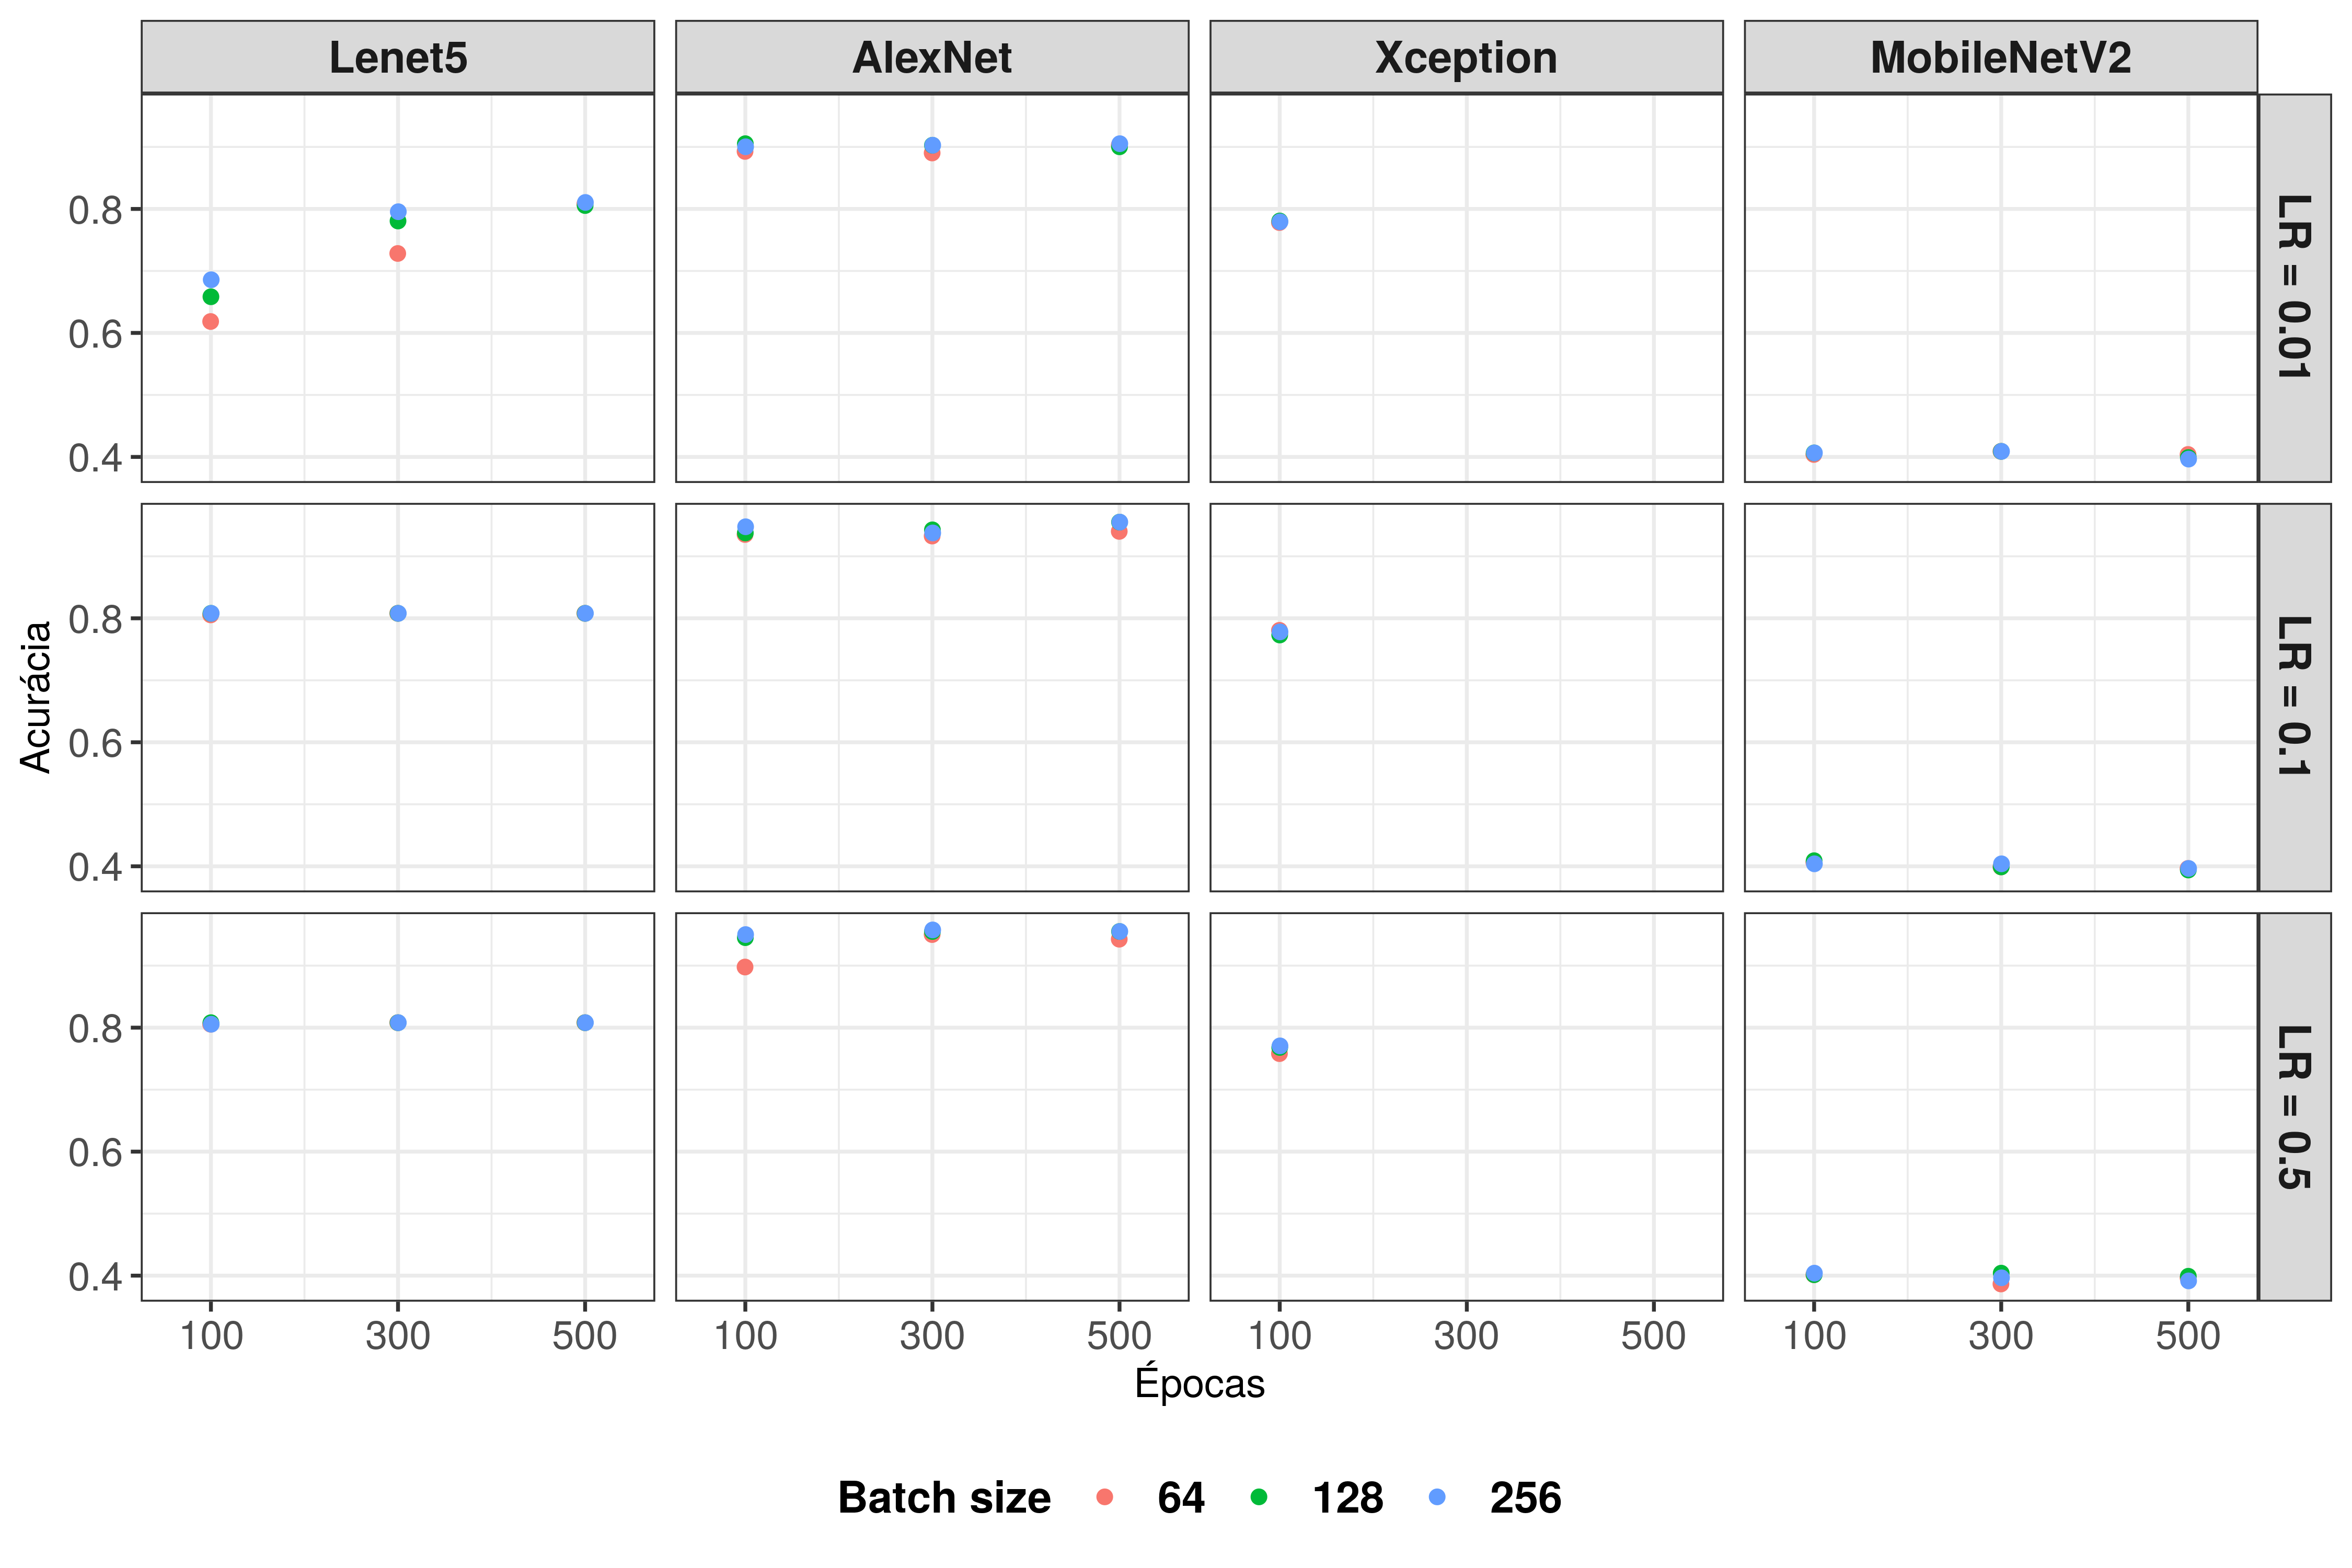
\includegraphics[width=1.6\textwidth]{/home/lacf14/machine_learning_ufpr/lab03/Analise/fig.png}
\caption{Acurácia observada para cada combinação do experimento.}
\end{figure}
\end{landscape}

\chapter{Considerações finais}
\label{cap:conclusao}

% ----------------------------------------------------------------------
% CAPÍTULO 5 - CONCLUSÃO
% ----------------------------------------------------------------------

Os resultados mostraram que a rede com melhor desempenho considerando acurácia como métrica de qualidade foi a AlexNet, com acurácias acima de 0.9. A segunda melhor rede foi a clássica Lenet5, com acurácias acima de 0.8. 

As redes pré treinadas Xception e MobileNetV2 foram problemáticas. A rede Xception mostrou-se a mais demorada para ajuste e não apresentou desempenho superior às redes Lenet5 e AlexNet; também devido ao tempo não foi possível obter as acurácias para os cenários com mais de 100 épocas de treinamento. A rede MobileNetV2 apresentou ajuste rápido para todas as épocas, contudo os resultados para esta rede em termos de predição se mostraram extremamente pobres.

A dificuldade em utilizar o modelo Xception se dá pelo tamanho e complexidade da rede. Além disso, trata-se de uma rede pré-treinada para classificar imagens em 1000 categorias de objetos, o que pode justificar um resultado não muito satisfatório para classificação de dígitos manuscritos.

Já a MobileNetV2 é um modelo de classificação desenvolvido pelo Google que fornece recursos para classificação em tempo real em smartphones, o que pode justificar a velocidade do ajuste mas pobreza dos resultados neste contexto específico.

Quanto à utilização da melhor rede AlexNet para geração de um vetor de características para regressão logística, notou-se que o resultado da regressão logística foi consideravelmente pior do que aquele observado na classificação com a própria rede neural convolucional. Enquanto a AlexNet atingiu acurácia acima de 0.9, o modelo de regressão logística com entrada cedida pela rede apresentou acurácia de aproximadamente 0.5.

A principal restrição deste estudo é o tamanho da base de treinamento. Como estamos utilizando redes neurais convolucionais, sabe-se que existe a necessidade de uma grande quantidade de dados para trabalhar. A alternativa sugerida para este cenário é utilizar técnicas de Data Augmentation. Contudo, devido ao tempo demandado pelo experimento e ao tempo de disponibilidade das GPUs na plataforma utilizada, não foi possível explorar esta alternativa. Mesmo assim, ressalta-se um resultado satisfatório da rede AlexNet, com acurácia acima de 0.9 e da Lenet5, capaz de atingir acurácias máximas de 0.8 em modelos que demandam pouco tempo, devido à simplicidade da rede.



% ---
\phantompart

% ---
% Conclusão
% ---

% ----------------------------------------------------------
% ELEMENTOS PÓS-TEXTUAIS
% ----------------------------------------------------------
\postextual

% ----------------------------------------------------------
% Referências bibliográficas
% ----------------------------------------------------------

%% Utilize este na elaboração do documento
\bibliography{refs}

%% Utilize este apenas ao final, quando não forem mais realizadas
%% alterações
% \begin{flushleft}
%   \small
% \renewcommand\refname{}
% \vspace*{-1.5cm}
% \input{01-tcc_corrigido.bbl}
% \end{flushleft}

% ----------------------------------------------------------
% Apêndices
% ----------------------------------------------------------

% ---
% Inicia os apêndices
% ---
% \begin{apendicesenv}

% Imprime uma página indicando o início dos apêndices
% \partapendices

% \chapter{Programas R}
% \label{capA:codigostcc}

% \end{apendicesenv}
% ---

% ----------------------------------------------------------
% Anexos
% ----------------------------------------------------------

%% % ---
%% % Inicia os anexos
%% % ---
%% \begin{anexosenv}
%% % Imprime uma página indicando o início dos anexos
%% \partanexos
%% \chapter{Lipsum}
%% \lipsum[30]
%% \end{anexosenv}

%---------------------------------------------------------------------
% INDICE REMISSIVO
%---------------------------------------------------------------------
% \phantompart
% \printindex
%---------------------------------------------------------------------

\end{document}
